\documentclass[
BCOR0.7cm,							% Bindekorrektur, bspw. 1 cm
]
{scrbook}

\newif\ifpdf
\ifx\pdfoutput\undefined
	\pdffalse              	%normales LaTeX wird ausgef�hrt
\else
	\pdfoutput=1           
	\pdftrue               	%pdfLaTeX wird ausgef�hrt
\fi

\ifpdf
	%\usepackage{ae}        % Benutzen Sie nur
	%\usepackage{zefonts}  	% eines dieser Pakete
\else
	%%Normales LaTeX - keine speziellen Fontpackages notwendig
\fi

\ifpdf %%Einbindung von Grafiken mittels \includegraphics{datei}
	\usepackage[pdftex]{graphicx} %%Grafiken in pdfLaTeX
\else
	\usepackage[dvips]{graphicx} %%Grafiken und normales LaTeX
\fi


\ifpdf
	\pdfinfo
	{
    /Author (Andreas �sterreicher)                                
    /Title (Admin)     
    /Subject (Administratorhandbuch)                                    
    /Keywords (ADMIN FH-Complete Technikum-Wien)
	}
\else			
\fi

\usepackage{listings} \lstset{numbers=left, numberstyle=\tiny, numbersep=5pt}
\lstset{language=tex} 


\usepackage[pdftex,colorlinks=true,urlcolor=blue,linkcolor=blue]{hyperref}
\usepackage[ngerman]{babel}		
\usepackage[T1]{fontenc}
\usepackage[latin9]{inputenc}
\usepackage{makeidx}
\usepackage{float}
\usepackage[small,bf]{caption}
\usepackage{fancyhdr}
\usepackage{amssymb,amsmath}
\makeindex

\graphicspath{{../../images/}}

\setlength{\tolerance}{2000}
\setlength{\parindent}{0pt}
\setlength{\parskip}{1ex plus 0.5ex minus 0.2ex}
\addtolength{\textheight}{2cm}
\addtolength{\headheight}{2pt}
\setlength{\captionmargin}{20pt}
\floatstyle{plain}
\floatname{example}{Example}

\newfloat{example}{hbtp}{loe}[chapter]
\floatplacement{figure}{hbtp}
\floatplacement{table}{htbp}

\newcommand{\dollar}{\char36}

\newenvironment{info}[1]{
    \hspace{-10mm}
    \fbox{
        \begin{minipage}{1cm}
        
\includegraphics[width=1cm]{icon_info}
        \end{minipage}
        \begin{minipage}{14.5cm}
        #1
        \end{minipage}
    }
}

\newenvironment{achtung}[1]{
    \hspace{-10mm}
    \fbox{
        \begin{minipage}{1cm}
        
\includegraphics[width=1cm]{icon_achtung}
        \end{minipage}
        \begin{minipage}{14.5cm}
        #1
        \end{minipage}
    }
}

\newenvironment{halt}[1]{
    \hspace{-10mm}
    \fbox{
        \begin{minipage}{1cm}
        
\includegraphics[width=1cm]{icon_halt}
        \end{minipage}
        \begin{minipage}{14.5cm}
        #1
        \end{minipage}
    }
}

\newenvironment{idee}[1]{
    \hspace{-10mm}
    \fbox{
        \begin{minipage}{1cm}
        
\includegraphics[width=1cm]{icon_idee}
        \end{minipage}
        \begin{minipage}{14.5cm}
        #1
        \end{minipage}
    }
}


\setlength{\unitlength}{1mm}

\newenvironment{markier}[5]{
    
    \thicklines \put(#2,#3){\vector(#4,#5){5}} \thinlines
    \put(#2,#3){\circle*{5}}
    \put(#2,#3){\textcolor{black}{\circle{5}}\makebox(-10,0){\textcolor{white}{#1}}}


}


\hyphenation{gleich-zeitig para-meter}


\begin{document}

\ifpdf
	\DeclareGraphicsExtensions{.pdf,.jpg,.png}
\else
	\DeclareGraphicsExtensions{.eps}
\fi

\pagestyle{fancyplain}
% Titelseite einbinden
%
% Titelseite, Abstrakt, Danksagung und Inhaltsverzeichnis
%
%% eigene Titelseitengestaltung %%%%%%%%%%%%%%%%%%%%%%%%%%%%%%%%%%%%%%%    

\begin{titlepage}
\begin{center}
\vspace*{40mm} \huge ADMIN-Handbuch\\
\vspace*{10mm}
\large \textsc{FH-Complete Administratorhandbuch}

\vfill 
\includegraphics[width=130mm]{fhcomplete}
	
\vfill \textsc{Technikum Wien}\\

Wien, \today
\end{center}
\end{titlepage}


\tableofcontents			% Inhaltsverzeichnis
\frontmatter					% Vorspann (z.B. r�mische Seitenzahlen)
\chapter{Einleitung}
\mainmatter						% Hauptteil

%% Kapitel Anfang %%%%%%%%%%%%%%%%%%%%%%%%%%%%%%%%%%%%%%%%%%%%%%%%%

\chapter{Subversion}
\label{Subversion}
Alle Dateien des FH-Complete Projektes werden in dem Versionsverwaltungstool Subversion abgelegt.
Die folgenden Subversion Repositories existieren:

\begin{tabular}{ll}
	https://www.fhcomplete.org/svn/fhcomplete & FH-Complete (extern erreichbar) \\
	https://www.fhcomplete.org/svn/wawi & WaWi (extern erreichbar, keine Schreibrechte) \\
	svn://calva.technikum-wien.at/fhcomplete & FH-Complete (nur intern) \\
\hspace*{22mm} /WAWI	 & WaWi alt \\
\hspace*{22mm} /WAWI2 & WaWi \\
\end{tabular}

\chapter{Installationsanleitung}
\label{Installationsanleitung - Client}
\section{Download von Seamonkey}
Zum Betrieb des FAS und Tempus wird ein Gecko basierter Browser ben�tigt. Die Applikation wurde auf der Seamonkey Suite entwickelt, l�uft aber auch unter MozillaSuite oder Firefox. Aktuelle Quellen des Seamonkey Browsers sind unter www.mozilla.org zu finden. Die Dialoge des Installationsassistenten k�nnen einfach mit 'Weiter' best�tigt werden. Der Standardpfad sollte unter Windows c:\textbackslash Programme\textbackslash mozilla.org\textbackslash seamonkey\textbackslash  sein.\\

\section{Download der Theme}
Die Theme(Skin) f�r Seamonkey ist im Grunde egal, jedoch unterst�tz die Calssic-Theme keine f�rbigen Buttons und teilweise kein Drag and Drop. Am besten eignet sich 'Orbit 3+1', es reicht aber auch die mitgelieferte Theme 'Modern'. Die Orbit 3+1 Theme ist im SVN unter portal/trunk/vilesci/admin/XPI/orbit-1.8f5-MiK.xpi zu finden. Zur Installation reicht es, das File in das Seamonkey Fenster zu ziehen und den aufscheinenden Dialog zu best�tigen.

\section{Einstellungen unter about:config}
Damit die Applikation reibungslos funktioniert m�ssen einige Sicherheitseinstellungen eingetragen werden.
�ffnen Sie dazu ein neues Browserfenster und geben Sie in die Adresszeile 'about:config' ein.\\
Im angezeigten Fenster m�ssen die folgenden Einstellungen ge�ndert werden.\\
- browser.cache.check\_doc\_frequency 1\\
- browser.cache.disk.capacity 0\\
- browser.downloadmanager.behavior 1\\
- dom.allow\_scripts\_to\_close\_windows true\\
- dom.disable\_window\_open\_feature.status false\\\
- signed.applets.codebase\_principal\_support true\\

Falls zum Versenden von Mails ein externer Mailclient verwendet wird (zB Outlook), muss ein neuer Wert unter about:config eingetragen werden.\\
Unter 'about:config' mit der rechten Maustaste ins leere klicken und new->boolean w�hlen:\\
network.protocol-handler.external.mailto true\\

\section{Seamonkey Bilder �ndern}
Um beim Starten der Applikation statt dem Seamonkey Logo das FH-Complete Logo anzuzeigen muss im Ordner c:\textbackslash Programme\textbackslash mozilla.org\textbackslash Seamonkey\textbackslash die Datei seamonkey.bmp mit dem FH-Complete Logo �berschrieben werden.\\
Um die Icons in der Titelleiste der Application zu �ndern, m�ssen die beiden Dateien tempus.ico und fas.ico (zu finden im SVN unter portal/trunk/skin/images/ )in den Ordner  c:\textbackslash Programme\textbackslash mozilla.org\textbackslash seamonkey\textbackslash chrome\textbackslash icons\textbackslash default\textbackslash  kopiert werden.

\section{Chrome Registrierung}
Ab Seamonkey und Firefox 1.5 m�ssen Applikationen die �ber .htaccess authentifizieren intern registriert werden. Hierzu gen�gt in klick auf https://vilesci.technikum-wien.at/vilesci/admin/XPI/FASoProduktiv/FASonline.xpi und dann auf Install.\\

\section{Verkn�pfung erstellen}
Zum Testen in der Adressleiste folgendes eingeben: chrome://fasonline/content/fasonline.xul\\

Wenn die Applikation ordnungsgem�� funktioniert, kann eine Verkn�pfung am Desktop angelegt werden:\\
C:\textbackslash Programme\textbackslash mozilla.org\textbackslash seamonkey\textbackslash seamonkey.exe -chrome chrome://fasonline/content/fasonline.xul

\section{Wichtige Hinweise}
FAS Benutzer m�ssen in der LDAP Gruppe HADESADM sein.
\chapter{Installationsanleitung - Server}
\label{Installationsanleitung - Server}
\section{Authentifizierung}
Derzeit wird die Authentifizierung der Benutzer gro�teils �ber HTTP Basic Authentifizierung durchgef�hrt. Dazu muss bei der Installation in den folgenden Ordnern ein .htaccess File angelegt werden:\\
- cis/private\\
- content\\
- include/tw\\
- system\\
- vilesci\\
\\
Die Authentifizierung des WaWi Systems erfolgt �ber Sessions.\\
\\

\section{Symbolische Links}
Es m�ssen einige Symbolische Links angelegt werden damit die Applikation ordnungsgem�� funktioniert:\\
- wawi/pdfExport.php zeigt auf content/pdfExport.php
\\



\chapter{Grundlegendes}
\label{Grundlegendes}
\section{Aufbau der Matrikelnummer}
\begin{figure}
	\centering
	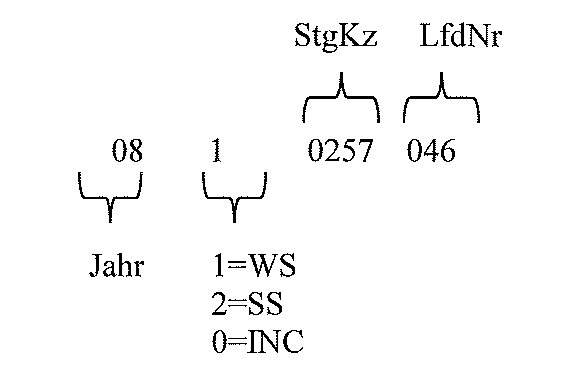
\includegraphics[width=0.75\textwidth]{Admin_AufbauMatrikelnummer.png}
	\caption{Aufbau der Matrikelnummer}
	\label{Aufbau der Matrikelnummer}
\end{figure}
Wenn an der dritten Stelle ein 2er steht (=SS) dann wird das Jahr um 1 verringert.

\section{Aufbau der UID}
\begin{figure}
	\centering
	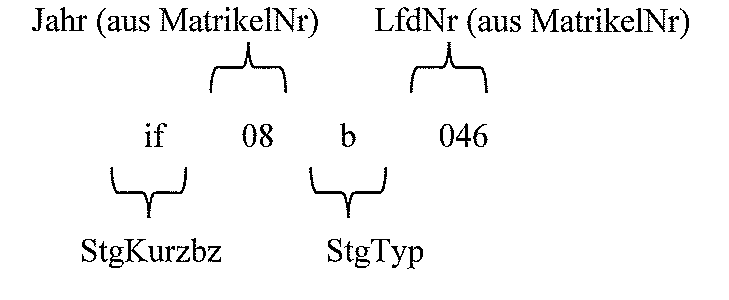
\includegraphics[width=0.75\textwidth]{Admin_AufbauUID.png}
	\caption{Aufbau der UID}
	\label{Aufbau der UID}
\end{figure}

\section{Variablen in public.tbl\_variable}
fas\_id - DEPRECATED\\
sleep\_time - DEPRECATED\\
\\
semester\_aktuell - Aktuell ausgew�hltes Studiensemester\\
kontofilterstg - wenn true dann werden nur die Buchungen des eigenen Studienganges angezeigt\\
emailadressentrennzeichen - Trennzeichen zwischen den Emailempf�ngern\\
\\
db\_stpl\_table - Studenplantabelle in die geschrieben wird (default: stundenplandev)\\
\\
ignore\_reservierung - Gibt an ob beim Verplanen im Stundenplan Reservierungen ignoriert werden sollen\\
ignore\_kollision - Gibt an ob beim Verplanen im Stundenplan Kollisionen ignoriert werden sollen\\
ignore\_zeitsperre - Gibt an ob beim Verplanen im Stundenplan Zeitsperren ignoriert werden sollen\\

\chapter{Berechtigung}
\label{Berechtigung}
Seit FHComplete 2.0 gibt es ein neues Berechtigungskonzept. Berechtigungen werden nun auf Organisationseinheiten aufgeh�ngt.
Wenn Personen Rechte auf eine Organisationseinheit zugeteilt bekommen, gelten diese auch
automatisch f�r die untergeordneten Organisationseinheiten. 
\section{Einzelberechtigungen}
Die Zuteilung der Berechtigungen f�r Personen erfolgt auf der Vilesci Seite unter Stammdaten->Berechtigungen\\
Berechtigungen k�nnen den Personen direkt zugeordnet werden. Hierbei muessen folgende Attribute ausgefuellt werden:\\
- berechtigung\_kurzbz\\
- uid\\
- oe\_kurzbz\\
- art\\
In diesem Fall bleiben die Felder rolle\_kurzbz und funktion\_kurzbz leer
\section{Rollenberechtigung}
Berechtigungen k�nnen zu Rollen zusammengefasst werden, um eine leichtere Verwaltung zu erm�glichen. (Assistenz, Adminstrator)
bei der Zuteilung einer Berechtigung zu einer Rolle muss die Art (in tbl\_rolleberechtigung) eingetragen werden. Die Tats�chlich 
verwendete Art, ist die Schnittmenge aus tbl\_rolleberechtigung.art und tbl\_benutzerrolle.art.\\
\\
Bei der Zuteilung von Rollen zu Personen sind folgende Felder auszuf�llen:\\
- rolle\_kurzbz\\
- uid\\
- oe\_kurzbz\\
Die Felder berechtigung\_kurzbz und funktion\_kurzbz bleiben leer.
\section{Funktionsberechtigung}
Zus�tzlich k�nnen Rechte Aufgrund von Benutzerfunktionen vergeben werden, um Beispielsweise alle Fachbereichskoordinatoren
bestimmte Rechte zuzuordnen.
Hier muss statt der UID die funktion\_kurzbz eingetragen werden. Das Feld oe\_kurzbz bleibt leer.
Bei der Pr�fung der Rechte, wird die oe\_kurzbz aus der Tabelle tbl\_benutzerfunktion herangezogen. Die Funktionen Mitarbeiter und Student sind nicht
extra in der Tabelle benutzerfunktion eingetragen sondern werden automatisch zugewiesen.\\
Die Zuteilung der Funktionsberechtigungen erfolgt auf der Vilesci Seite unter Personen->Funktionen->Berechtigung\\
\section{Negativrechte}
Alle Berechtigungen und Rollen k�nnen auch als Negativrecht eingetragen werden. Hierbei muss das Feld negativ auf true gesetzt werden.
Dies kann dazu ben�tzt werden, um bei der Zuteilung einer gesamten Rolle, der Person wieder einzelne Rechte zu entziehen.

\section{Aufbau}
Berechtigungen sind nach einem bestimmten Schema aufgebaut:\\
\textbf{lehre/lehrveranstaltung}\\
\textbf{lehre/lehrveranstaltung:begrenzt}\\
Zuerst wird das Modul genannt in dem die Berechtigung zum Tragen kommt. Durch einen '/' getrennt folgt der Name der Berechtigung. Die Berechtigung kann durch ':' in Unterberechtigungen unterteilt werden. 

\achtung{\textbf{Wichtig} Wenn eine Person die Berechtigung f�r 'lehre/lehrveranstaltung' hat, dann hat sie auch automatisch die Rechte f�r die Berechtigung 'lehre/lehrveranstaltung:begrenzt'.}\\

\section{Webservice/SOAP Schnittstellen}
Da die Webserivce Schnittstellen auch f�r Studierendenprojekte verwendet werden, k�nnen hier die Rechte noch detaillierter verwaltet werden.
Die Leserechte der Webservices k�nnen auf einzlene Attribute eingeschr�nkt werden.
Die Zugriffssteuerung dazu erfolgt in der Datenbank �ber die Tabelle system.tbl\_webservicerecht.
Hier kann folgendes angegeben werden:\\
\\
- F�r welche Berechtigung wird das Webservicerecht erteilt (berechtigung\_kurzbz)\\
- Welche Webservice Methode betrifft das Recht (methode)\\
- Welches Attribut dieser Methode darf angezeigt werden (attribut)\\
\\
F�r jedes Attribut das angezeigt werden soll, ist eine eigene Zeile in die Tabelle einzuf�gen.
Attribute die nicht in dieser Tabelle aufscheinen, werden aus dem Webservice Response entfernt.\\
Auf diese Weise k�nnen eigene eingeschr�nkte Berechtigungen auf Webservices erstellt werden.\\
\\

\chapter{Cronjob}
\label{Cronjob}
\\
Um die Daten regelm��ig zu Pr�fen und um Inkonsistenzen vorzubeugen, k�nnen im FH-Complete Zeitgesteuerte Scripte (Cronjobs) gestartet werden.
Cronjobs werden im FHComplete gesammelt verwaltet. Damit diese funktionieren, muss in der Crontab folgender Eintrag angelegt werden:\\
\\
*/5   *   * * *    /var/www/vilesci/htdocs/vilesci/cronjobs/cronjob.php > cron.log\\
\\
Dieser Eintrag muss auf jedem Server gemacht werden, auf dem ein Job laufen soll.\\
Die einzelnen Jobs k�nnen �ber die Vilesci-Seite unter Admin->Cronjobs verwaltet werden.
Zum Testen ob der Dienst funktioniert existiert ein Testjob. Dieser sendet automatisch ein Mail wenn der Job gestartet wird.
\\
\\
\textbf{Folgende Felder k�nnen zu Cronjobs eingetragen werden:}\\
- Titel: Titel des Jobs\\
- Beschreibung: Kurzbeschreibung zu dem Job\\
- Server: Server auf dem der Job ausgef�hrt werden soll (Crontab-Eintrag muss auf diesem Server vorhanden sein!)\\
- Datei: absoluter Pfad zu dem Cronjob. Beispiel f�r den Testjob: '/var/www/vilesci/htdocs/vilesci/cronjobs/testjob.php'\\
- Zeitangabe: der Ausf�hrungszeitpunkt kann entweder direkt oder als Interval angegeben werden. (mit */<Zeitinterval) Die Funktionsweise ist mit jener 
der Unix Cronjobs vergleichbar.\\
Beispiele:
Job soll jeden 1. des Monats um 02:00 Uhr gestartet werden:\\
Das Feld Tag muss auf 1 gesetzt werden, Stunde auf 2 und Minute auf 00. Die anderen Felder bleiben leer.\\
Job soll jeden 2. Tag laufen:\\
Das Feld Tag wird auf */2 gesetzt. Alle anderen bleiben leer.\\
Der Job soll jeden Sonntag im Jahr 2010 um 01:00 Uhr laufen:\\
Jahr wird auf 2010 gesetzt, Wochentag auf Sonntag, Stunde auf 1 und Minute auf 00. Die restlichen Felder bleiben leer.\\
- Aktiv: inaktive Jobs werden nicht ausgef�hrt\\
- Standalone: Wenn dies gesetzt ist, dann darf der Job nur alleine ausgef�hrt werden. Wenn zur selben Zeit ein anderer Job l�uft, dann wird dieser nicht ausgef�hrt.\\
- Reihenfolge: Bei Jobs die zur gleichen Zeit gestartet werden, werden die mit der niedrigeren Reihenfolge zuerst ausgef�hrt.\\
- Varialben: Hier k�nnen Variablen eingetragen werden, die an den Cronjob �bergeben werden. Diese m�ssen im JSON-Format eingetragen werden. Zu unterst�tzung steht ein Variablen-Editor zur Verf�gung.
Beim Anlegen eines neuen Jobs k�nnen die Variablen automatisch initialisiert werden. Dies ruft den Cronjob mit einem Initialisierungsparameter auf. Das Script setzt daraufhin die Standard-Variablen f�r diesen Job.
\\


\chapter{Assistenz}
\label{ToDo zum Anlegen einer neuen Assistenz}
Die folgenden Schritte sind n�tig um eine neue Assistenz im System anzulegen:\\
- Account anlegen\\
- Account zur Gruppe hadesadm hinzuf�gen\\
- Berechtigung unter Vilesci->Stammdaten->Berechtigung hinzuf�gen\\
- Variablen unter vilesci->Stammdaten->Variablen mit Standardwerten anlegen\\
- In der Tabelle Studiengang die EMail-Adresse der Assistenz eintragen\\
- Benutzerfunktion Assistenz unter Vilesci->Benutzer->Funktion hinzuf�gen\\

\chapter{LVPlanung}
\label{LVPlanung}
Wenn der Lektor bei einer Lehrveranstaltung ge�ndert wird, \\
und diese Lehreinheit schon im LV-Plan verplant ist, \\
wird der Eintrag automatisch im LV-Plan aktualisiert sofern folgende Kriterien erf�llt sind:\\
- ignore\_kollision=false\\
- es entsteht keine Kollision im LV-Plan durch diese �nderung\\

\section{Anzeigen des Pers�nlichen LV-Planes eines Studenten}
Um im CIS den Pers�nlichen Stundenplan eines Studenten anzuzeigen ist wie folgt vorzugehen:\\
- Rechte Maustaste auf den eigenen Pers�nlichen LV-Plan\\
- 'Link in neuem Fenster �ffnen' ausw�hlen\\
- in der Adresszeile die pers\_uid auf die UID des Studenten �ndern\\
- zus�tzlich den Parameter '\&type=student' anh�ngen\\
\chapter{Mailverteiler}
\label{Mailverteiler}
Die Mailverteiler werden t�glich neu erstellt. Hierzu werden Textfiles mit den entsprechenden Verteilern erstellt. Dies erfolgt durch die Scripten im Verzeichnis system/mlists.

Verteiler die Automatisch erstellt werden, haben in der Gruppe das Attribut generiert auf true gesetzt.\\
(Hier werden die Personen automatisch zugeteilt �ber das Script system/mlists/mlists\_generate.php)\\

\label(Sperrung von Mailverteilern)
Mailverteiler k�nnen gesperrt werden, damit diese nur von Mitarbeitern verwendet werden k�nnen.\\
Dazu muss im config die Konstante MAILVERTEILER\_SPERRE auf true gesetzt sein. Zur Benutzung des Verteilers muss dieser dann erst Freigeschalten werden. Dies erfolgt �ber das kleine Symbol links neben dem Verteilernamen. \\
Das Symbol zur Entsperrung eines Verteilers erscheint nur dann, wenn aktiv=false ist.\\

(Diese Schritte zeigen nur die Einstellungen im FH-Complete damit der Verteiler als gesperrt angezeigt wird. Die tats�chliche Sperre der Verteiler muss extra am MailServer eingerichtet werden.)\\

\section{Alias}
Vom System werden automatisch Email-Aliase angelegt. Diese werden mit vorname.nachname@domain generiert. Wenn der Alias bereits vergeben ist, wird kein Ersatz generiert.\\
Die Email-Aliase werden f�r alle Benuzter angelegt (auch f�r Studenten).\\
Das Erstellen von Aliase f�r Studenten kann auch unterbunden werden, wenn in der Datei /include/globals.inc.php der Studiengang f�r den keine Aliase erstellt werden sollen, zu dem Array 'noalias' hinzugef�gt wird.\\
\\
Die Aliase werden in die Datei tw\_alias.txt exportiert.
\chapter{Urlaubstool}
\label{Urlaubstool}
Es besteht die M�glichkeit, als Administrator die Urlaubsverwaltung aller Mitarbeiter im CIS einzusehen.
Dazu muss die Benutzerrolle admin angelegt sein.\\
Um die Zeitsperren anzuzeigen muss an die URL der Parameter ?uid=xxx angehaengt werden.\\
Dies funktioniert bei den Files \\
- urlaubsfreigabe.php\\
- zeitsperre\_resturlaub.php\\
\chapter{Erweiterbarkeit}
\label{Erweiterbarkeit}

Es gibt die M�glichkeit, das Programm zu erweitern, ohne dabei gr��ere Probleme bei Updates zu verursachen. \\
\\
Teile des Programmcodes wurden in das Verzeichnis /trunk/include/tw/ ausgelagert um individuelle Anpassungen am Programm durchzuf�hren. (zB Men�struktur des CIS, Vorlagen f�r PDFs die nicht �ber XSLT erstellt werden, ...)
Dieser Ordner kann kopiert und unter einem anderen Namen im include Ordner abgelegt werden. Der Pfad zu diesem Ordner wird im config.inc.php in
der Konstante EXT\_FKT\_PATH abgelegt. Danach k�nnen die Dateien in diesem Verzeichnis abge�ndert werden, ohne das diese bei einem Update �berschrieben werden.\\

\section{Zus�tzliche Men�punkte im FAS-Online}
Im FAS-Online k�nnen auch zustzliche Men�punkte eingef�gt werden, ohne dass diese bei einem Update �berschrieben werden. Dies ist n�tzlich falls zus�tzliche Statistiken o.�. eingebaut werden sollen. Dazu gibt es im Ordner /trunk/include/tw/ zwei Files:\\
- fas\_zusatzmenues.inc.php\\
- fas\_zusatzmenues.js.php\\
\\
Im ersten File kann der XUL Code f�r die Erstellung zus�tzlicher Men�s eingetragen werden.\\
Das Zweite File enth�lt den dazugeh�rigen Javascript Code um etwa die Seite mit der Statistik aufzurufen.\\
\\
Einen Beispielcode f�r das Hinzuf�gen eines neuen Men�punktes befindet sich in den oben genannten Dateien.\\
\\
Der neue Men�punkt wird im FAS, nach einf�gen des Codes, automatisch vor dem Men�punkt Extras eingebunden.
\chapter{PDF-Generierung}
\label{PDF-Generierung}
PDFs werden im System �ber XSLT Vorlagen erzeugt. \\
Dazu wird zuerst eine XSLT Vorlage mit einer XML Datei in ein XSL-FO Dokument umgewandelt.
Aus diesem XSL-FO Dokument wird anschlie�en das PDF erzeugt.

\begin{figure}
	\centering
	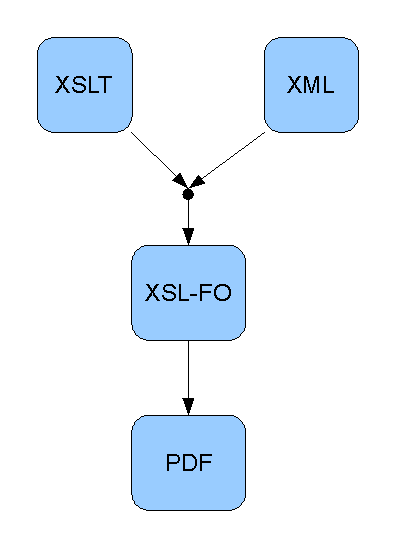
\includegraphics[width=0.30\textwidth]{Admin_PdfGenerierung.png}
	\caption{Pdf-Generierung}
	\label{Pdf-Generierung}
\end{figure}

Die XSLT Vorlagen werden in der Datenbank gespeichert und k�nnen pro Studiengang unterschiedlich sein.\\
Die zugeh�rige XML Datei wird von den Scripten im RDF Verzeichnis erstellt.\\
\\
\achtung{\textbf{Wichtig} Damit der Server die PDFs generieren kann, muss dieser ohne Authentifizierung auf das RDF-Verzeichnis zugreifen k�nnen.
Dies muss gesondert in den Einstellungen des Webservers eingetragen werden. \\
Ab Apache 2.2 kann dies auch per .htaccess eingestellt werden}\\


\chapter{BIS-Meldung}
\section{Mitarbeiter}
\subsection{Ablauf}
Es gibt die M�glichkeit, die BIS-Meldung des Vorjahres zu importieren. Dies ist Hilfreich, wenn die Meldung zum Ersten mal mit dem FAS erstellt wird, damit die Daten nicht h�ndisch eingetragen werden m�ssen. Dies geschieht �ber den Men�punkt BIS->Mitarbeiter->Import.\\
\\
�ber den Men�punkt BIS->Mitarbetier->checkVerwendung kann gepr�ft werden, ob alle Mitarbeiter eine g�ltige BIS-Verwendung eingetragen haben. Die aufscheinenden Fehler sollten vor der BIS-Meldung bereinigt werden.\\
\\
Wenn die Fehler in checkVerwendung behoben wurden, kann checkFunktion aufgerufen werden. Dieses Script erstellt die BIS-Funktionen. Hierbei wird die Anzahl der Stunden anhand der Lehrauftr�ge zu den Verwendungen hinzugef�gt.\\
\\
Nach diesen Schritten, kann die Meldung �ber den den Men�punkt 'Meldung generieren' erstellt werden.
\subsection{Inaktive Studieng�nge}
Bei der Personalmeldung d�rfen keine Studiengangsleiter von Studieng�ngen gemeldet werden, die keinen Unterricht mehr haben. Diese Studieng�nge k�nnen aber nicht immer deaktiviert werden (z.B. wenn noch Diplomanden vorhanden sind ohne Abschlusspr�fung). Diese Studieng�nge m�ssen in der Datei /vilesci/bis/personalmeldung.php in das Array \$nichtmelden eingetragen werden.

%% Kapitel Ende   %%%%%%%%%%%%%%%%%%%%%%%%%%%%%%%%%%%%%%%%%%%%%%%%%
\appendix							% Beginn des Anhangs
\chapter{Schluss}
\listoftables					% Tabellenverzeichnis
\listoffigures				% Abbildungsverzeichnis
\end{document}
